Para poder realizar los estudios requeridos se hace necesario acceder a la información contenida en los archivos $*.root$ de forma eficiente, la descripción del contenido del árbol de datos de nuestros archivos se puede observar en el enlace \url{https://cp3.irmp.ucl.ac.be/projects/delphes/wiki/WorkBook/RootTreeDescription}. Pero se hace necesario un interpretador externo al entorno predeterminado de \textbf{ROOT} para poder acceder a la infomación pertinente a la investigación, de aquí que se programe una clase en python que permita de forma cómoda extraer información para adaptarla según las necesidades que puedan surgir (se hace uso de las paqueterías \texttt{pyroot}). Esta clase (ver Fig. \ref{class_darksusy1}) además de permitir acceder a los datos, procesa la información para hacer la reconstrucción más probable de la masa del fotón oscuro partiendo de la información muónica, el diagrama de la figura muestra el procedimiento utilizado.

\begin{figure}[h]
\centering
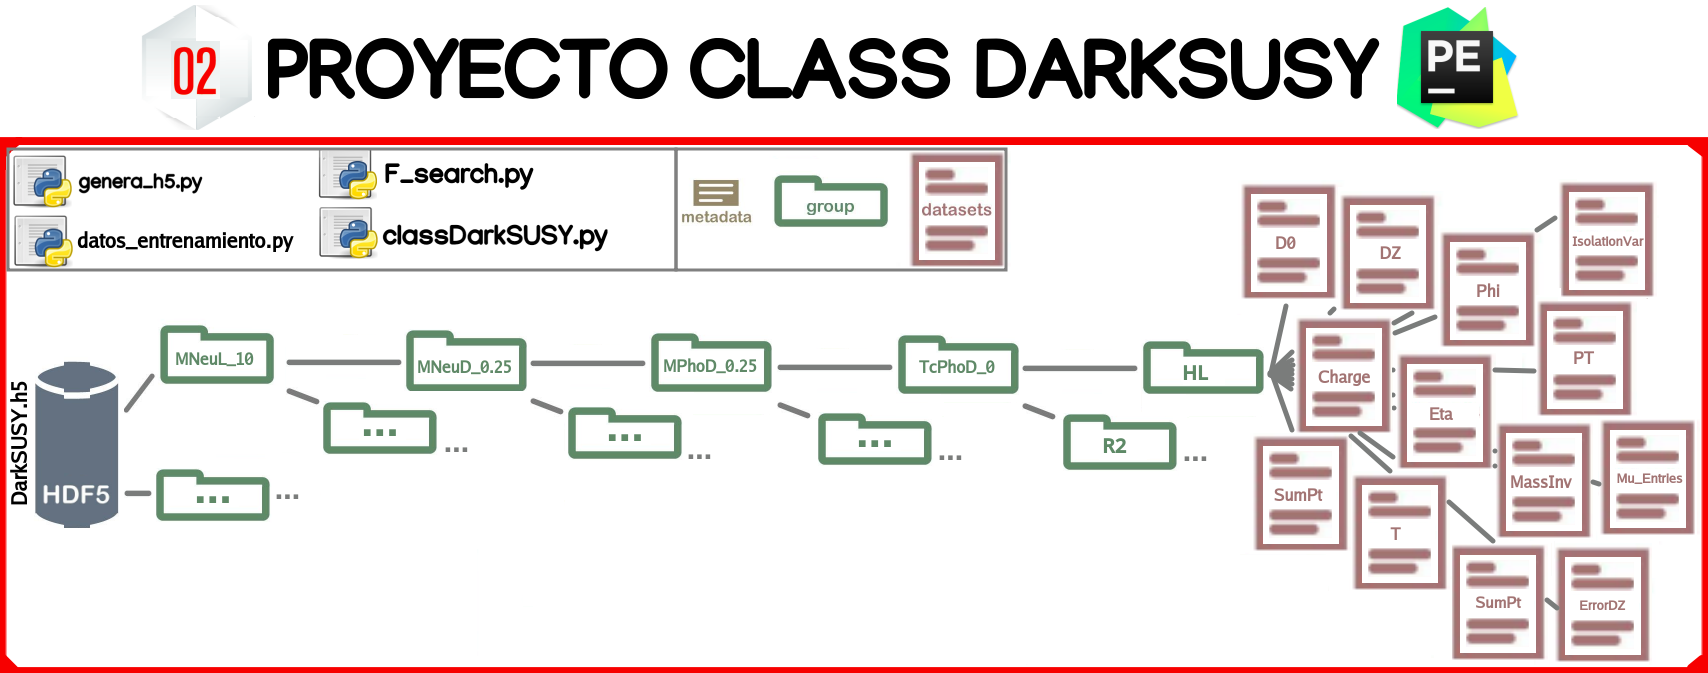
\includegraphics[width=.9\textwidth]{Simulacion/imagenes/class_darksusy.png}
\caption{Estructura del proyecto interpretador de la información contenida en los archivos $*.root$. Pagina del proyecto \url{https://github.com/franky8939/DarkSUSY/blob/master/modules/darkSUSY/classDarkSUSY.py}}
\label{class_darksusy1}
\end{figure}

Dada la gran cantidad de información y archivos a procesar para el análisis estadístico incluso ante un acceso eficiente, la gran dispersión de la información hace que los procesos de recolección de datos sea lento y con altos requerimientos de memoria, la forma en que se abordo esta dificultad fue incorporar la información solicitada en un mismo archivo de tipo \textbf{HDF5} (\textbf{H}ierarchical \textbf{D}ata \textbf{F}ormat) la cual posee una librería de propósito general con un formato de ficheros para el almacenaniento de datos científicos. 
\begin{figure}[h]
\centering
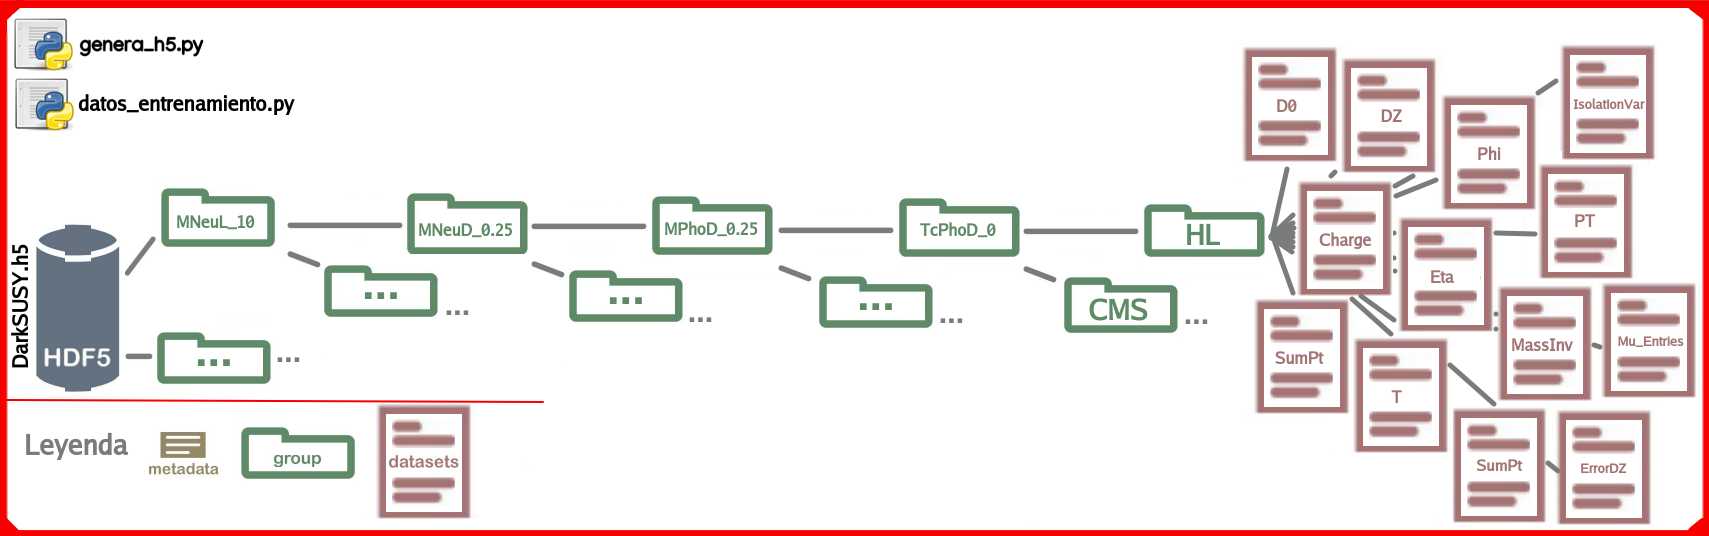
\includegraphics[width=1\textwidth]{Simulacion/imagenes/class_darksusy3.png}
\caption{Estructura de los metadatos con la información filtrada. Pagina del proyecto \url{https://github.com/franky8939/DarkSUSY/blob/master/00-Convertidores/genera_h5.py}}
\label{class_darksusy2}
\end{figure}

Este formato de datos \textbf{HDF5} fue creado para atender las necesidades de científicos e ingenieros que trabajan en entornos de computación de altas prestaciones que requieran un uso intensivo de datos, de aquí que este predeterminado para que sea muy eficiente en el almacenaniento y el acceso. 